\documentclass[12pt]{article}
\usepackage{fullpage}
\usepackage[top=10mm, bottom=45mm, left=10mm, right=10mm]{geometry}
\usepackage{amsmath,amsthm,amssymb}
\usepackage{lastpage}
\usepackage{enumerate}
\usepackage{fancyhdr}
\usepackage{xcolor}
\usepackage{graphicx}
\usepackage{listings}
\usepackage{hyperref}
\usepackage{answers}
\usepackage{setspace}
\usepackage{enumitem}
\usepackage{multicol}
\usepackage{mathrsfs}
\usepackage{algorithmic}
\usepackage{stmaryrd}
\usepackage[ruled,linesnumbered,vlined]{algorithm2e}
\usepackage{tikz}
 \usepackage{fancyvrb}
\usetikzlibrary{automata, positioning}
\usepackage{minted}



\hypersetup{%
  colorlinks=true,
  linkcolor=blue,
  linkbordercolor={0 0 1}
}

\lstdefinestyle{Python}{
    language        = Python,
    frame           = lines, 
    basicstyle      = \footnotesize,
    keywordstyle    = \color{blue},
    stringstyle     = \color{green},
    commentstyle    = \color{red}\ttfamily
}

\setlength{\parindent}{0.0in}
\setlength{\parskip}{0.05in}

\newcommand\course{\textbf{EE 456}}   
\newcommand\name{Aishwarye Omer}     

\pagestyle{fancyplain}
\headheight 35pt
\lhead{\name\\\course{}}
\chead{\textbf{\Large Homework - 08}}
\rhead{\today}
\lfoot{}
\cfoot{}
\rfoot{\small\thepage}
\headsep 1.5em

\newlength\myindent
\setlength\myindent{2em}
\newcommand\bindent{%
  \begingroup
  \setlength{\itemindent}{\myindent}
  \addtolength{\algorithmicindent}{\myindent}
}
\newcommand\eindent{\endgroup}
\definecolor{codegreen}{rgb}{0,0.6,0}
\definecolor{codegray}{rgb}{0.5,0.5,0.5}
\definecolor{codepurple}{rgb}{0.58,0,0.82}
\definecolor{backcolour}{rgb}{0.95,0.95,0.92}

%Code listing style named "mystyle"
\lstdefinestyle{mystyle}{
	backgroundcolor=\color{backcolour},   commentstyle=\color{codegreen},
	keywordstyle=\color{magenta},
	numberstyle=\tiny\color{codegray},
	stringstyle=\color{codepurple},
	basicstyle=\ttfamily\footnotesize,
	breakatwhitespace=false,         
	breaklines=true,                 
	captionpos=b,                    
	keepspaces=true,                 
	numbers=left,                    
	numbersep=5pt,                  
	showspaces=false,                
	showstringspaces=false,
	showtabs=false,                  
	tabsize=2
}

%"mystyle" code listing set
\lstset{style=mystyle}

\newenvironment{solution}[1][Solution]{\begin{trivlist}
\item[\hskip \labelsep {\bfseries #1}]}{\end{trivlist}}


\begin{document}

\textbf{Question: Give a graph of Y as time varies from -1 to 1 for the network given}

\BlankLine
\BlankLine

\textbf{Solution:} The source code followed by the graph:\BlankLine\BlankLine

\begin{lstlisting}[language=Python]
import numpy as np
import math
from matplotlib import pyplot as plt
	
v = np.asmatrix([[1.12, 0.36],[2.46, 0.27],[6.11, 0.09],[-1.08, 0.28],[0.96, 0.24],[-1.03, -0.29],[-0.58, 0.12],[-1.11, -0.34],[1.13,0.05],[1.05,0.06]])
w = np.asmatrix([[-1.35],[0.14],[4.26],[1.18],[-1.02],[1.20],[0.55],[1.37],[-1.27],[-1.20],[0.45]])
output = []
input = np.linspace(-1,1,10000) 
	
for i in input:
	#calulating hidden output
	y=0 
	hidden_output = [] 
		for item in v:
			h = i * item[0, 0] + item[0, 1] 
			h = 2/(1+np.exp(-h))-1 
			hidden_output.append(h)
		#calculating final output   
		
		for j in range(0,10):
			y = y + hidden_output[j] * w.item(j)
			final_output = y + w.item(w.size-1) 
			final_output = 2/(1+np.exp(-final_output))-1 
	output.append(final_output)

\end{lstlisting}

\begin{lstlisting}
fig = plt.figure()
axes = fig.add_axes([0.1,0.1,1.1,1.1]) 
plt.plot(input, output)
plt.grid()
plt.xlabel('time', fontsize=12) 
plt.ylabel('y', fontsize=12) 
plt.savefig('foo.png', bbox_inches='tight') 
plt.show()
\end{lstlisting}


	
\begin{center}
	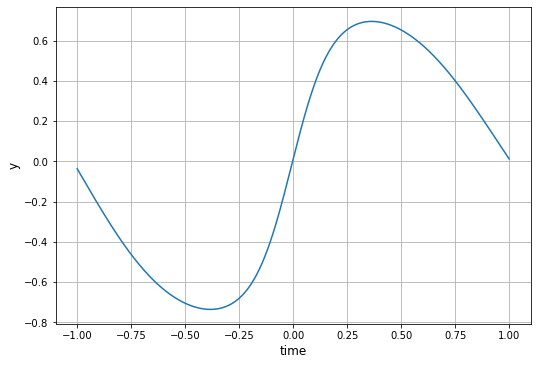
\includegraphics{output_2_0.png}
\end{center}


\end{document}